\clearpage
%%=========================================
\section{MCT Film Grown by LPE on Substrate A}\label{sec:subAc}

Nomarski optical microscopy images reveal that the surface of the \ac{mct} film has wavy structures with a large number of circular features, as seen in Fig.~\ref{fig:subAc_om}. 

\begin{figure}[htbp]
    \centering
    \mySubfigure{0.31\textwidth}{LPE453_nomarski_grid_16_20x.jpg}[fig:subAc_om_centre][angle=180]
    \hfill
    \mySubfigure{0.31\textwidth}{LPE453_nomarski_grid_18_20x.jpg}[fig:subAc_om_edge][angle=180]
    \hfill
    \mySubfigure{0.31\textwidth}{LPE453_nomarski_grid_07_20x.jpg}[fig:subAc_om_corner][angle=180]
    \caption[Nomarski phase contrast microscopy images of \ac{mct} film grown by \ac{lpe} on substrate A.]{Nomarski phase contrast microscopy images of \ac{mct} film grown by \ac{lpe} on (111)B-oriented substrate A: \subref{fig:subAc_om_centre} Near the centre; \subref{fig:subAc_om_edge} near the right edge; and \subref{fig:subAc_om_corner} near the upper right corner.}
    \label{fig:subAc_om}
\end{figure}

%%=========================================
\subsection{Particles and Surface Features}
%Seven different types of particles and surface features were observed on the surface of substrate B, see Fig.~\ref{fig:subBa_sem_w_eds}. They will be described and identified in the following.
Four different types of particles are observed on the surface of substrate A after surface pre-growth preparation, see Fig.~\ref{fig:subAb_sem_w_eds}. They will be described and identified in the following.

%The presence of depressions or voids, which may, or may not, retain droplets of solution, can be interpretated according to the results published by Bauser [9, E. Bauser, AppI. Phys. 15 (1978) 243]. The presence on the substrate of defects like oxide, microprecipitates, graphite particles prevents the wetting of the substrate by the liquid phase and can induce voids or depressions.Fig. 6 illustrates this mechanism.

The density of donut shaped structures was found to be between \SIrange{4e+3}{6e+4}{\centi\metre^{-2}}. The mean void density was \SI{2e+04}{\centi\metre^{-2}} with a standard deviation of \SI{1e+04}{\centi\metre^{-2}}. A graphical representation of the density at different locations on the film can be seen in Fig.~\ref{fig:LPE453_densityData}.

\begin{figure}[htbp]
    \centering
    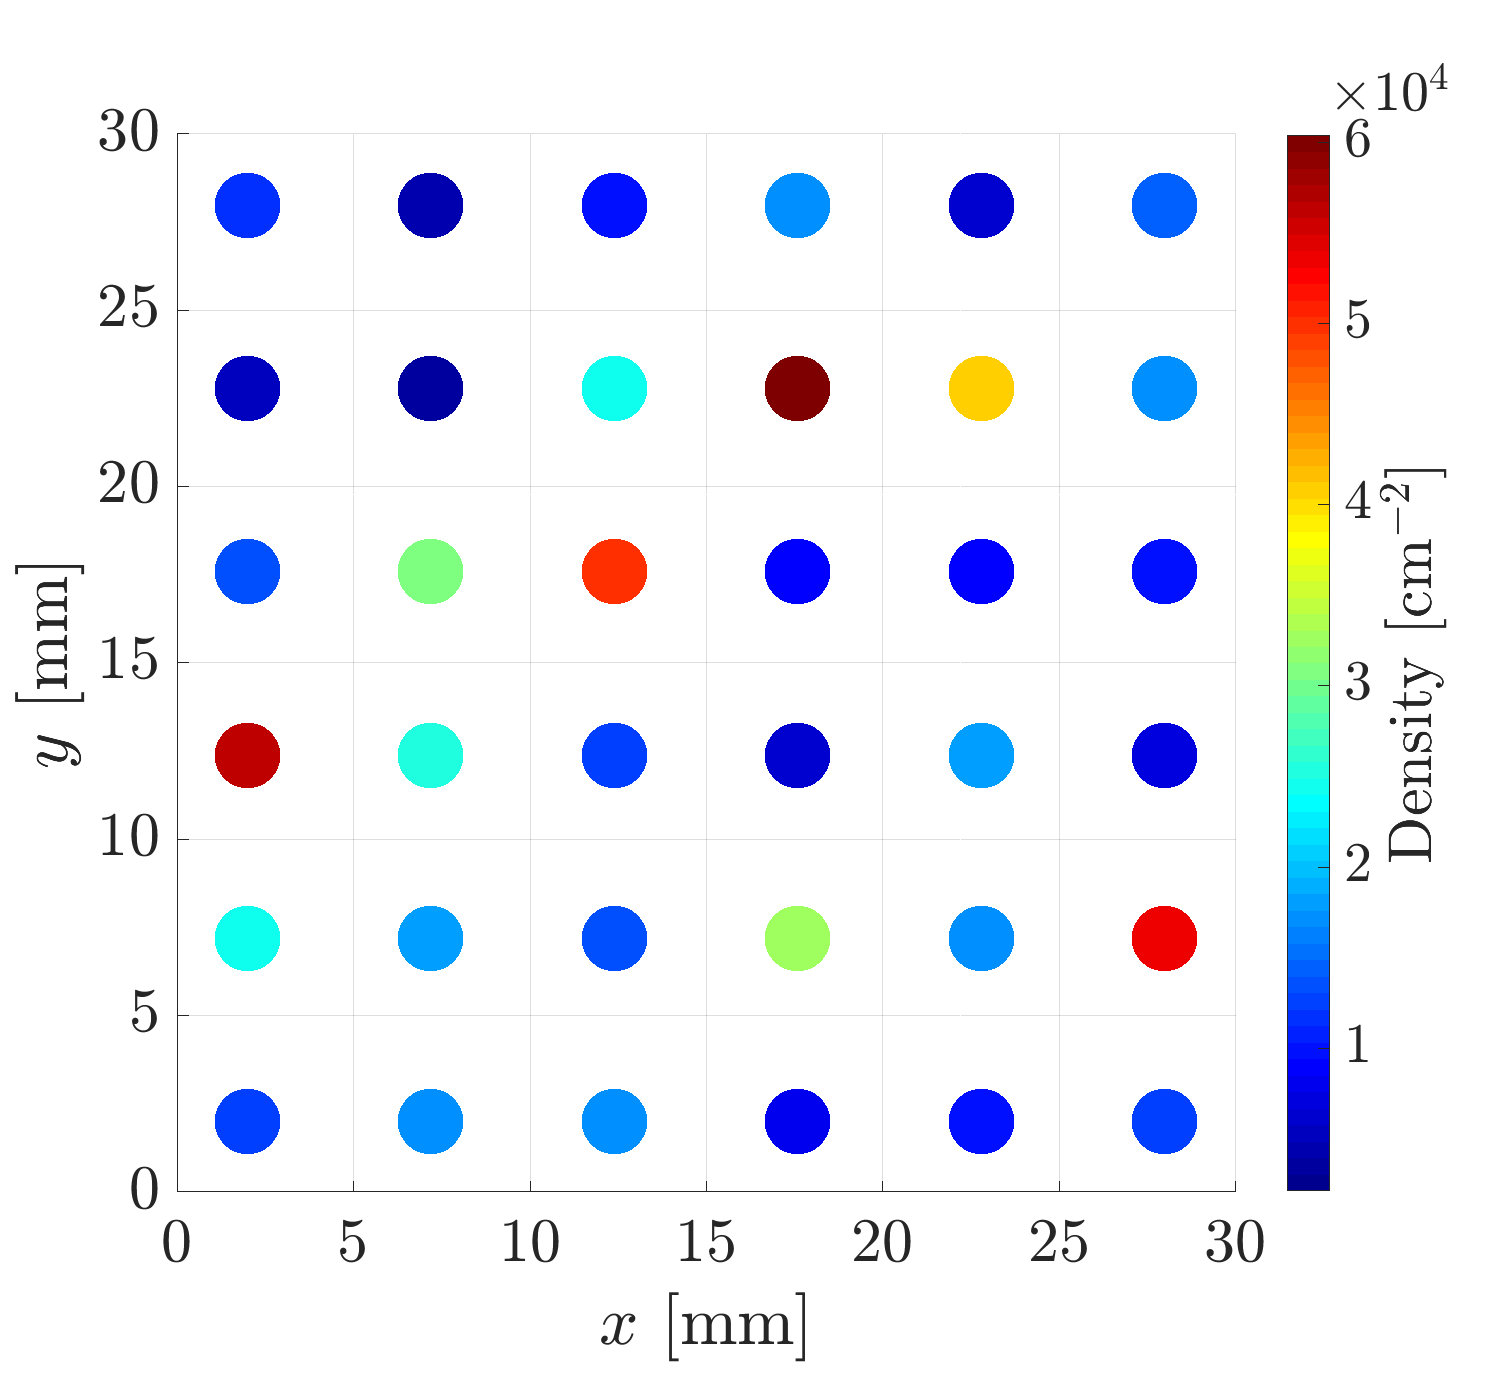
\includegraphics[width=0.5\linewidth]{LPE453_densityData.png}
    \caption[Map of the density of donut shaped structures on the \ac{mct} film grown on substrate A.]{A map of the density of donut shaped structures at 36 different locations on the $\SI{30}{\milli\metre}\times\SI{30}{\milli\metre}$ \ac{mct} film grown on substrate A. The density was observed to vary between \SIrange{4e+3}{6e+4}{\centi\metre^{-2}} with an average defect density of \SI{2e+04}{\centi\metre^{-2}}.}
    \label{fig:LPE453_densityData}
\end{figure}

%%=========================================
%\subsection{Surface Roughness}

%%=========================================
\subsection{Impurity Analysis}

%%=========================================